\documentclass[11pt]{article}
\usepackage{graphicx}
\usepackage{caption}
\usepackage[a4paper, top=1in, bottom=1.1in, left=1in, right=1in]{geometry}
\usepackage[utf8]{inputenc} % utf8
\usepackage[T1]{fontenc}
\usepackage{xcolor}
\usepackage{listings}
\usepackage{subcaption}
\usepackage{siunitx}\usepackage{wrapfig}
\usepackage{varioref}\usepackage{amsmath}
\usepackage{commath}


\setlength{\belowcaptionskip}{-6pt}
\makeatletter
\lst@Key{matchrangestart}{f}{\lstKV@SetIf{#1}\lst@ifmatchrangestart}
\def\lst@SkipToFirst{%
  \lst@ifmatchrangestart\c@lstnumber=\numexpr-1+\lst@firstline\fi
  \ifnum \lst@lineno<\lst@firstline
  \def\lst@next{\lst@BeginDropInput\lst@Pmode
    \lst@Let{13}\lst@MSkipToFirst
    \lst@Let{10}\lst@MSkipToFirst}%
  \expandafter\lst@next
  \else
  \expandafter\lst@BOLGobble
  \fi}
\makeatother

\lstset{  
  backgroundcolor=\color{gray!30},   % choose the background color; you must add \usepackage{color} or \usepackage{xcolor}
  basicstyle=\footnotesize,        % the size of the fonts that are used for the code
  breakatwhitespace=false,         % sets if automatic breaks should only happen at whitespace
  breaklines=true,                 % sets automatic line breaking
  captionpos=t,                    % sets the caption-position to bottom
  escapeinside={\%*}{*)},          % if you want to add LaTeX within your code
  extendedchars=true,              % lets you use non-ASCII characters; for 8-bits encodings only, does not work with UTF-8
  frame=single,                   % adds a frame around the code
  keepspaces=true,                 % keeps spaces in text, useful for keeping indentation of code (possibly needs columns=flexible)
  keywordstyle=\color{blue},       % keyword style
  language=C++,                 % the language of the code
  numbers=left,                    % where to put the line-numbers; possible values are (none, left, right)
  numbersep=20pt,                   % how far the line-numbers are from the code
  numberstyle=\tiny\color{gray}, % the style that is used for the line-numbers
  rulecolor=\color{blue!20},       
  showspaces=false,                % show spaces everywhere adding particular underscores; it overrides 'showstringspaces'
  showstringspaces=false,          % underline spaces within strings only
  showtabs=false,                  % show tabs within strings adding particular underscores
  stepnumber=1,                    % the step between two line-numbers. If it's 1, each line will be numbered
  tabsize=2,                   % sets default tabsize to 2 spaces
  language=Octave,
  framesep=7pt,
  xleftmargin=12pt,
  xrightmargin=11pt
}

\setlength{\fboxsep}{4pt}
\DeclareCaptionFormat{myformat}{%
  \hspace{1pt}\fcolorbox{blue!20}{gray!20}{\footnotesize\parbox{\dimexpr\textwidth-17pt\fboxsep\fboxrule\relax}{#1#2\ttfamily#3}}\vspace{-4pt}
}
\captionsetup[lstlisting]{format=myformat}
\captionsetup[figure]{labelfont=sf,hypcap=false,format=hang,margin=0.5cm,justification=RaggedRight,calcwidth=0.7\linewidth,font=footnotesize,justification=justified}
\captionsetup[table]{labelfont=sf,hypcap=false,format=hang,margin=1cm,justification=RaggedRight,calcwidth=0.8\linewidth,font=footnotesize,justification=justified}
\labelformat{equation}{(#1)}

%%% Local Variables:
%%% mode: latex
%%% TeX-master: t
%%% End:

%%% Math typesetting macros
\newcommand{\di}[2]{#1_\textup{#2}} % Descriptive Index: Macro for quick upright index (as opposed to a variable index, which should be italic) %% Separate file for preamble with macros and stuff
\renewcommand{\lstlistlistingname}{Code listings}

%% Title
\title{Laboration 1: PID-controls\\ {\small Sensors and Sensing}}
\author{Michael Flo{\ss}mann, Tom Olsson}
\date{\today}

\begin{document}
\maketitle %Title area
\begin{center}
  \emph{All code for this exercise can be found at \\ \url{https://github.com/tgolsson/sensors-arduino-lab1}}
\end{center}
\lstlistoflistings % List of all code snippets
\listoffigures % List of all figures
\listoftables
\lstset{ matchrangestart=t} %initialise the linerange-macro for \lstinput...
\section{Theory and motivation}
Control algorithms are important to create predictable, safe, and reliable operation in robotics applications. Two important algorithms/controllers for this purpose is the \emph{PID-controller} and the \emph{mimimum jerk trajectory}. 

\subsection{PID controller}
PID in the name PID-controller is short for \emph{Proportional}-\emph{Integral}-\emph{Derivative}-controller. As this implies, the controlling signal is based on a proportion of the current error, the previous error, and the rate of change of the observed error. The mathemathical formulation of this can be seen in \vref{eq:pid}.\par \vspace{10pt}
{\footnotesize
  \begin{tabular}{l l l}
    \textbf{Let:} \\
 &$e(t)$ &be some error measurement between current state and preferred state\\
 &$\di{K}{p}$, $\di{K}{i}$, $\di{K}{d}$ &be the respective weights for the proportional, integral and derivate terms \\
 &$u(t)$ &be the output signal at time \emph{t} \\
    \textbf{Then:}
  \end{tabular}
  \begin{align}
    u(t) &= \di{K}{p}\cdot e(t) + \di{K}{i} \cdot\int_{0}^{t}e(\tau)\cdot \dif\tau + \di{K}{d} \cdot \od{e(t)}{t}\label{eq:pid}
  \end{align}}
\par

\subsection{Minimum jerk}
\label{sec:mje}
The minimum jerk equation is an important part of creating smooth control. When a rotating actuator such as a motor starts, both the rotor and the stator will be at rest. The momentum generated by the motor can therefore cause movement in either part. As this can create an unwanted jerk while the rotor accelerates, it is important to accelerate slowly so that the stator remains at rest in relation to the reference frame. This can be achieved by the \emph{minimum jerk equation} shown in \vref{eq:mje}.
\par \vspace{10pt}
{\footnotesize
  \begin{tabular}{l l l}
    \textbf{Let:} \\
 &$\di{x}{i}$, $\di{x}{f}$ &be the initial and final states\\
 &$t$, $T$ &be the elapsed time since the action started, and the preferred total time for the action  \\
 &$x(t)$ &be the estimated state at time \emph{t} \\
    \textbf{Then:}
  \end{tabular}
  \begin{align}
    x(t) &= \di{x}{i} +  (\di{x}{f} - \di{x}{i}) \cdot \left[10\left(\frac{t}{T}\right)^3 - 15\left(\frac{t}{T}\right)^4 + 6\left(\frac{t}{T}\right)^6 \right]\label{eq:mje}          
  \end{align}}
The $T$ parameter has to be estimated. If $T$ is much larger than  the actual time that is needed for the trajectory, the velocity will be very low, and if $T$ is too low $x(t)$ will approach infinity unless $\frac{t}{T}$ is clamped to $[0,1]$. However, this solution is not optimal. Instead, we choose to calculate the optimal time $\di{T}{opt}$ as follows.%, and this can be seen in \ref{eq:derivative}.
\par
For finding out the optimal time $\di{T}{opt}$, we substitute:
{
  \footnotesize
\begin{align}
  \label{eq:tau_substitution}
  \hfill\tau:&=\frac{t}{T}\\
  \ref{eq:mje}\Rightarrow \hspace{50pt} x(\tau)&= \di{x}{i} +  (\di{x}{f} - \di{x}{i}) \cdot \left(10\tau^3 - 15\tau^4 + 6\tau^6 \right)\\
   \od{x(\tau)}{\tau}&= (\di{x}{f} - \di{x}{i})\cdot\left(30\tau^2-60\tau^3+36\tau^5\right)\label{eq:dx_dtau}\\
  \intertext{\normalsize \ref{eq:dx_dtau} reaches its' maximum at $\tau=0.5$ (proof trivial) with the value:}
  \eval{\od{x(\tau)}{\tau}}_{\tau=0.5}&=\frac{15}{18}\cdot(\di{x}{f} - \di{x}{i})\label{eq:dx_1518} \\
\intertext{\normalsize In order to make this term dependent on $T$, we must resubstitute \vref{eq:tau_substitution} into \vref{eq:dx_1518}.}
  \ref{eq:tau_substitution}\Rightarrow \hspace{63pt}%\od{\tau}{t}
\dot{\tau}
&=\frac{1}{T}\\
  \Rightarrow\hspace{58pt}\dif\tau&=\dif t\cdot\frac{1}{T}\label{eq:dtau_resubs}\\
  \ref{eq:dx_dtau},\ref{eq:dtau_resubs}\Rightarrow\hspace{24pt}%\eval{T\cdot\od{x(\tau)}{t}}_{\tau=0.5}&=\frac{15}{18}\cdot(\di{x}{f} - \di{x}{i})\\
%  &\Rightarrow
\eval{\od{x(\tau)}{t}}
%\dot{\tau}}
_{\tau=0.5}&=\frac{15}{18}\cdot\frac{\di{x}{f} - \di{x}{i}}{T}\label{eq:dx_dt}\\
\intertext{\normalsize Now, if we state an optimal maximum velocity $\di{v}{opt}$ for the minimum jerk equation, we can calculate the optimal time $\di{T}{opt}$ for this velocity.}
  \Rightarrow\hspace{25pt}\eval{\od{x(\tau)}{t}}_{\tau=0.5}&=\di{v}{opt}\\
  \ref{eq:dx_dt}\Rightarrow\hspace{52pt} \di{T}{opt}&=\frac{15}{18}\cdot\frac{\di{x}{f} - \di{x}{i}}{\di{v}{opt}}\label{eq:t_opt}
\end{align}
}\par

\section{Implementation}
The purpose of this exercise is to implement a PID-controller using the minimum jerk trajectory, and use this implementation for both a \emph{set-position} mode of operation, as well as a \emph{set-velocity} mode of operation. An important part of this exercise is the tuning of the PID-parameters for either mode of operation. \par

\subsection{Hardware and environment}
The laboration is performed using an \emph{Arduino Due} microcontroller, with the \emph{Arduino Motor Shield R3}. These are programmed using Serial-over-USB; with the dedicated IDE. The version of the IDE used is 1.6.5. The exercise also includes usage of the \emph{Robot Operating System} [ROS], version \emph{Indigo Igloo}. \par

The motor used is the \emph{Micro Motors RHE158 75:1 12V DC}, connected to the motor shield. As the USB-bus cannot supply enough power to drive the motor, an external 12V power adapter was used.
\paragraph{Measurements}
In order to ensure correct behaviour, the amount of tics per revolution as well as the maximum velocity of the motor was measured and compared to the datasheet \cite{datasheet_motor_1},\cite{datasheet_motor_2}. \par
\begin{table}[!htbp]
  \centering
  \caption{Measured and expected motor characteristics}
  \begin{tabular}{l|cc}
    Characteristic & Datasheet & Measured \\ \hline
    Ticks/rotation & 230.5 &235.0\\ 
    Ticks/second & 311.0 & 280.0\\
    Rotations/second & 1.35 & 1.19
  \end{tabular}
  \label{tab:measurements}
\end{table}
The maximum speed in the data sheet refers to the motor speed without load. Since there was load present at the laboratory outset, the measured value of ticks per second was used. The ticks per rotation value was measured turning a varying amount of ticks and seeing when one rotation was completed. This method is expected to be relatively uncertain, since there is a large possible error margin without proper measuring equipment. In order to improve the measurement, 10 rotations were made, and the result was verified twice. \par

The ticks per second value for maximum speed was measured by applying a duty cycle of 100\% to the PWM and programatically measuring the ticks. Ten measurements were made for 10 seconds each, and the average ticks per second was chosen as the speed value. This measurement is considered very exact and is used in the rest of this paper. 

\subsection{Position controller}
The first part of the position is the callback for setting a target position. This code is shown in listing \vref{lst:position-callback}. The code updates the mode of operation, and sets the start and end position for the movement. The integral term of the controller is also set to zero. Tests were made without setting it to zero, but this caused unreliable behaviour in some situations, such as when the target position was moved closer to the current position. \par

As can be seen on line 319, \ref{eq:t_opt} from subsection \vref{sec:mje} is used to calculate the end time point. This ensures that we  reach the maximum speed at $\frac{t}{T} = 0.5$. While this is suboptimal for long trajectories, it makes sure that $T$ is realistic for shorter paths. If long trajectories will be the normal mode of operation; an approach with splines should be used instead of the minimun jerk equation. \par
\newpage
\lstinputlisting[label=lst:position-callback,caption={Set Position Callback}, linerange={307-324 }]{../lab1_stub/lab1_stub.ino}

The position controller is implemented to setup the parameters for PID and MJE. The code for this can be see in listing \vref{lst:position-controller}. The minimum jerk function is called with start-time, current time, and end-time, as well as start and end position. The output of this equation is then used to calculate the momentary error, as well as its derivative. These are then given to the PID-controller. \par

\lstinputlisting[label=lst:position-controller,caption={Position Controller},linerange={221-249}]{../lab1_stub/lab1_stub.ino}

\subsection{Velocity controller}
As with the position controller, an important part of the velocity controller is the callback for setting the target velocity. This code is shown in listing \vref{lst:velocity-callback}. The only difference to the position callback is the $T$ parameter. This was tested to see the minimum acceptable time to go from full forward speed to full reverse speed, and 3 seconds seemed to be a reasonable value. As the difference in speed is 560 ticks per second; this therefore becomes $\left\lceil\frac{3}{560}\right\rceil _4 = 0.006$. \par

\lstinputlisting[label=lst:velocity-callback,caption={Set Velocity Callback},linerange={333-351}]{../lab1_stub/lab1_stub.ino}

The velocity controller is also very similar to the position controller, as can be seen in listing \vref{lst:velocity-controller}. As before, the minimum jerk function is called with start-time, current time, and end-time. However, the last two parameters are replaced by  start and end velocity. As can be seen on line 254-255 the momentary velocity is smoothed using a sliding sum, and normalized to seconds. The reason for this is that the maximum speed of the motor is 235 ticks per second, while the program operates at 1 kHz. The general rule therefore is that no encoder ticks will happen during one program cycle, therefore causing the momentary speed to be measured as 0. After this, the velocity controller continues as the position controller


\lstinputlisting[label=lst:velocity-controller,caption={Velocity Controller},linerange={252-273}]{../lab1_stub/lab1_stub.ino}

\subsection{PID-controller, minimum jerk and actuation}
The PID-controller used before matches the equation shown earlier in \vref{eq:pid}. The implementation is shown in listing \vref{lst:pid}.

\lstinputlisting[label=lst:pid,caption={PID-implementation},linerange={285-294}]{../lab1_stub/lab1_stub.ino}

The mimimum jerk equation is also implemented as shown earlier  in \vref{eq:mje}. The only difference is that the fraction $\frac{t}{T}$ is clamped to $[0,1]$. Though this should not be needed with the guarantees made by the calculations of $T$, it was put in as a safeguard. Otherwise, a delayed controller can potentially accumulate an infinite error can lose control. The code for this can be seen in listing \vref{lst:mje}.\par

\lstinputlisting[label=lst:mje,caption={Mimimum jerk implementation},linerange={277-283}]{../lab1_stub/lab1_stub.ino}

Lastly, the actuation function is what actually transforms the control value into a PWM output. The function receives the output from the PID-controller, and clamps it to the allowed range as well as setting the direction of the motor. The code for this can be seen in listing \vref{lst:actuate}.

\lstinputlisting[label=lst:actuate,caption={Actuator implementation},linerange={208-219}]{../lab1_stub/lab1_stub.ino}


\section{Verification and results}
\subsection{PID-tuning}
The tuning of the PID-controller was done in three steps. First, the $k_p$ term was found with which reasonable behaviour was seen. Then, the $k_i$ term was estimated to be on the order of $\num{1e-6}$, based on $dT=1000$. This follows from the definition of the integral. When a good value was found, the derivative term was increased and was estimated to be on the order of magnitude $\num{1e0}$. This follows from the definition of the derivative term and the timestep. Lastly, several tests were ran with the final configuration to make sure that no erroneous behaviour was occuring. \par

After testing, the values $k_p = 60$, $k_i = \num{1e-6}$, and $k_d = 2$ was found to provide the best performance. These parameters were found to provide good results for both velocity and position control. Plots of the behaviours can be seen in figs. \ref{fig:pos} and \vref{fig:vel}. \par

\begin{figure}[h]
  \centering
  \begin{subfigure}[b]{.9\textwidth}
    \centering
    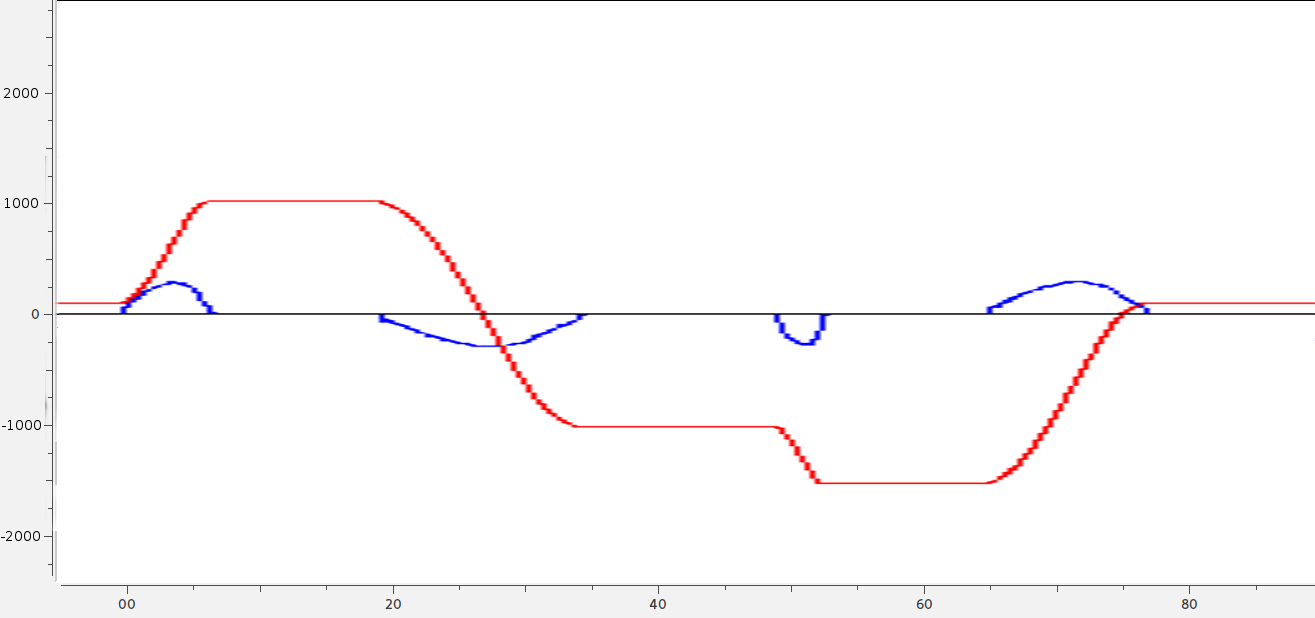
\includegraphics[width=.9\textwidth]{figures/posplot.png}
    \caption{\scriptsize Plot of target position := $[{1000}, {-1000}, {-1500}, 50]$}\label{fig:pos}\vspace{20pt}
  \end{subfigure} 
  \begin{subfigure}[b]{.9\textwidth}
    \centering
    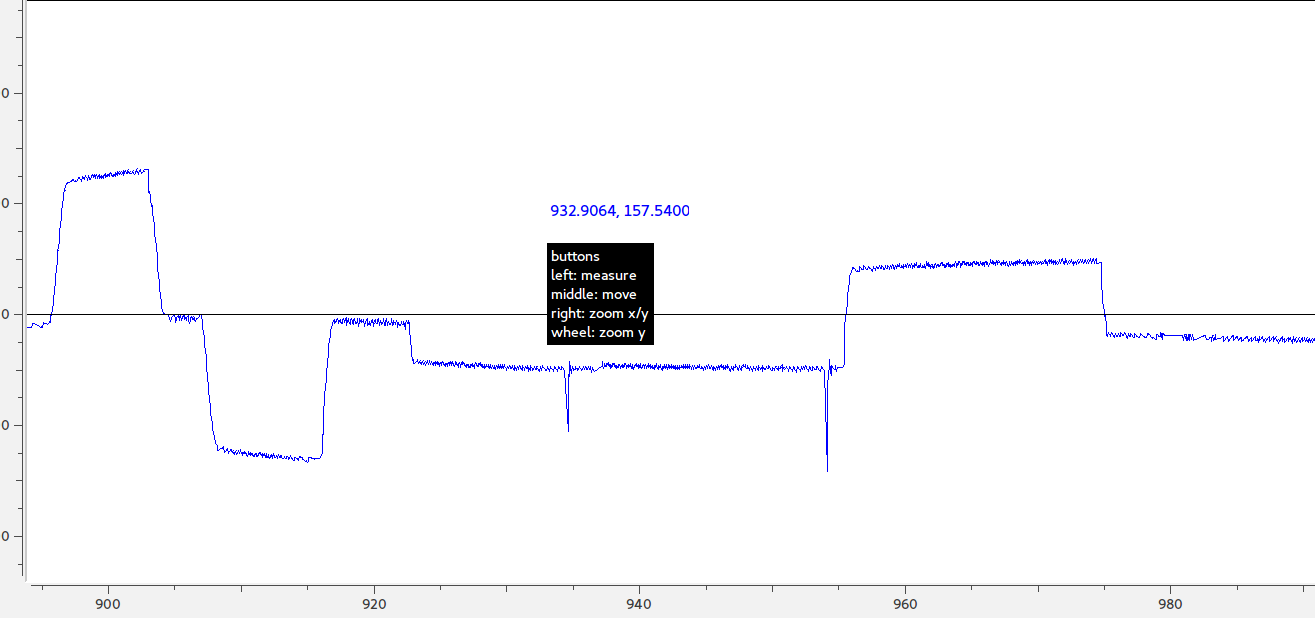
\includegraphics[width=.9\textwidth]{figures/velplot.png}
    \caption{\scriptsize Plot of target velocity := $[280, {-10}, {-280}, {-20}, {-100}, 100, {-50}]$. The spikes are believed to be caused by speed difference between microcontroller execution (1 kHz) and maximum encoder speed (235 ticks/second). There is no visible change in output however, and the spikes only last 2-3 ms.}    \label{fig:vel}
  \end{subfigure}
  \captionof{figure}[Plots of controller behaviour]{Plots of controller behaviour for some target values.}
\end{figure}
\subsection{Results}
A PID controller controlling the angle and angular speed of a DC motor with tick-counter was created. It was implemented using an \emph{Arduino Due} along with ROS. Both angle and velocity control show the expected behaviour, including a minimum jerk motion for the angle control.\par
LThe angle control is carried out in the optimal time of the minimum jerk equation. For bigger angles to traverse, this timeframe is relatively long. By replacing the minimum jerk equation with other models which also lower the motor jerk but remaining at maximum speed for longer times (i.e. spline interpolation), the efficiency could be vastly increased on this part.

\begin{thebibliography}{99}
\bibitem{datasheet_motor_1} RH158 micro motor \url{http://www.reductor-motor.com/eng-micRH158.htm} (accessed at 2015-11-22)
\bibitem{datasheet_motor_2} gear-motors with Hall-effect encoder \url{http://www.reductor-motor.com/eng-mic_e_data1.htm} (accessed at 2015-11-22)
\end{thebibliography}

\end{document}



%%% Local Variables:
%%% mode: latex
%%% TeX-master: t
%%% End:
